Voice-based interfaces are becoming really popular in recent years. They are not only integrated with mobile devices (Apple Siri, Google Assitant) but also deployed for entire voice-first systems (Amazon Echo, Google Home). According to VoiceLabs's report \cite{VoiceLabs:2017}, there were 1.7 million voice-first devices shipped in 2015. In 2016, this figure were 6.5 million and is predicted to be 24.5 million this year. The potential to build applications on top of these interfaces seems limitless. For example, we can directly use voice to order the device to play music, read a newspaper, turn on/off the light and other linked devices in our house. My project is focused on robotic applications, especially for controling robot's movement, recognizing and finding objects. These visual applications are developped using state-of-the-art deep neural network algorithms. The project involves numerous interesting problems in artificial intelligence such as speech recognition, information extraction, image classification and object detection.


%The general objective is to build a voice system that transfers voice commands to text, then extracts the information from text and maps to corresponding robot actions (figure \ref{fig:diagramSystem}). A more ambitious goal is to illustrate an interactive learning process of the robot. This will be tackled during the project.
%\begin{figure}[tb]
%	\centering
%	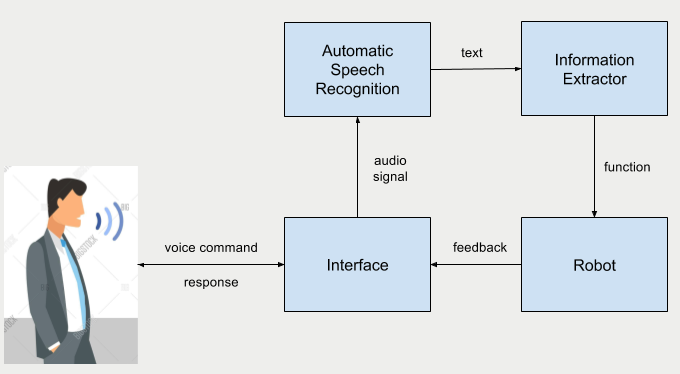
\includegraphics[width = 0.7\hsize]{./figures/diagramSystem}
%	\caption{Diagram of the system}
%	\label{fig:diagramSystem}
%\end{figure}